\documentclass[12pt,a4paper]{article}

\usepackage[a4paper,text={16.5cm,25.2cm},centering]{geometry}
\usepackage{lmodern}
\usepackage{amssymb,amsmath}
\usepackage{bm}
\usepackage{graphicx}
\usepackage{microtype}
\usepackage{hyperref}
\setlength{\parindent}{0pt}
\setlength{\parskip}{1.2ex}

\hypersetup
       {   pdfauthor = { Kevin Corcoran },
           pdftitle={Assignment 4},
           colorlinks=TRUE,
           linkcolor=black,
           citecolor=blue,
           urlcolor=blue
       }

\title{Assignment 4}

\author{ Kevin Corcoran }

\usepackage[makeroom]{cancel}

\usepackage{import}
\usepackage{pdfpages}
\usepackage{transparent}
\usepackage{xcolor}

\newcommand{\incfig}[2][1]{%
    \def\svgwidth{#1\columnwidth}
    \import{./figures/}{#2.pdf_tex}
}

\pdfsuppresswarningpagegroup=1

\usepackage{upquote}
\usepackage{listings}
\usepackage{xcolor}
\lstset{
    basicstyle=\ttfamily\footnotesize,
    upquote=true,
    breaklines=true,
    breakindent=0pt,
    keepspaces=true,
    showspaces=false,
    columns=fullflexible,
    showtabs=false,
    showstringspaces=false,
    escapeinside={(*@}{@*)},
    extendedchars=true,
}
\newcommand{\HLJLt}[1]{#1}
\newcommand{\HLJLw}[1]{#1}
\newcommand{\HLJLe}[1]{#1}
\newcommand{\HLJLeB}[1]{#1}
\newcommand{\HLJLo}[1]{#1}
\newcommand{\HLJLk}[1]{\textcolor[RGB]{148,91,176}{\textbf{#1}}}
\newcommand{\HLJLkc}[1]{\textcolor[RGB]{59,151,46}{\textit{#1}}}
\newcommand{\HLJLkd}[1]{\textcolor[RGB]{214,102,97}{\textit{#1}}}
\newcommand{\HLJLkn}[1]{\textcolor[RGB]{148,91,176}{\textbf{#1}}}
\newcommand{\HLJLkp}[1]{\textcolor[RGB]{148,91,176}{\textbf{#1}}}
\newcommand{\HLJLkr}[1]{\textcolor[RGB]{148,91,176}{\textbf{#1}}}
\newcommand{\HLJLkt}[1]{\textcolor[RGB]{148,91,176}{\textbf{#1}}}
\newcommand{\HLJLn}[1]{#1}
\newcommand{\HLJLna}[1]{#1}
\newcommand{\HLJLnb}[1]{#1}
\newcommand{\HLJLnbp}[1]{#1}
\newcommand{\HLJLnc}[1]{#1}
\newcommand{\HLJLncB}[1]{#1}
\newcommand{\HLJLnd}[1]{\textcolor[RGB]{214,102,97}{#1}}
\newcommand{\HLJLne}[1]{#1}
\newcommand{\HLJLneB}[1]{#1}
\newcommand{\HLJLnf}[1]{\textcolor[RGB]{66,102,213}{#1}}
\newcommand{\HLJLnfm}[1]{\textcolor[RGB]{66,102,213}{#1}}
\newcommand{\HLJLnp}[1]{#1}
\newcommand{\HLJLnl}[1]{#1}
\newcommand{\HLJLnn}[1]{#1}
\newcommand{\HLJLno}[1]{#1}
\newcommand{\HLJLnt}[1]{#1}
\newcommand{\HLJLnv}[1]{#1}
\newcommand{\HLJLnvc}[1]{#1}
\newcommand{\HLJLnvg}[1]{#1}
\newcommand{\HLJLnvi}[1]{#1}
\newcommand{\HLJLnvm}[1]{#1}
\newcommand{\HLJLl}[1]{#1}
\newcommand{\HLJLld}[1]{\textcolor[RGB]{148,91,176}{\textit{#1}}}
\newcommand{\HLJLs}[1]{\textcolor[RGB]{201,61,57}{#1}}
\newcommand{\HLJLsa}[1]{\textcolor[RGB]{201,61,57}{#1}}
\newcommand{\HLJLsb}[1]{\textcolor[RGB]{201,61,57}{#1}}
\newcommand{\HLJLsc}[1]{\textcolor[RGB]{201,61,57}{#1}}
\newcommand{\HLJLsd}[1]{\textcolor[RGB]{201,61,57}{#1}}
\newcommand{\HLJLsdB}[1]{\textcolor[RGB]{201,61,57}{#1}}
\newcommand{\HLJLsdC}[1]{\textcolor[RGB]{201,61,57}{#1}}
\newcommand{\HLJLse}[1]{\textcolor[RGB]{59,151,46}{#1}}
\newcommand{\HLJLsh}[1]{\textcolor[RGB]{201,61,57}{#1}}
\newcommand{\HLJLsi}[1]{#1}
\newcommand{\HLJLso}[1]{\textcolor[RGB]{201,61,57}{#1}}
\newcommand{\HLJLsr}[1]{\textcolor[RGB]{201,61,57}{#1}}
\newcommand{\HLJLss}[1]{\textcolor[RGB]{201,61,57}{#1}}
\newcommand{\HLJLssB}[1]{\textcolor[RGB]{201,61,57}{#1}}
\newcommand{\HLJLnB}[1]{\textcolor[RGB]{59,151,46}{#1}}
\newcommand{\HLJLnbB}[1]{\textcolor[RGB]{59,151,46}{#1}}
\newcommand{\HLJLnfB}[1]{\textcolor[RGB]{59,151,46}{#1}}
\newcommand{\HLJLnh}[1]{\textcolor[RGB]{59,151,46}{#1}}
\newcommand{\HLJLni}[1]{\textcolor[RGB]{59,151,46}{#1}}
\newcommand{\HLJLnil}[1]{\textcolor[RGB]{59,151,46}{#1}}
\newcommand{\HLJLnoB}[1]{\textcolor[RGB]{59,151,46}{#1}}
\newcommand{\HLJLoB}[1]{\textcolor[RGB]{102,102,102}{\textbf{#1}}}
\newcommand{\HLJLow}[1]{\textcolor[RGB]{102,102,102}{\textbf{#1}}}
\newcommand{\HLJLp}[1]{#1}
\newcommand{\HLJLc}[1]{\textcolor[RGB]{153,153,119}{\textit{#1}}}
\newcommand{\HLJLch}[1]{\textcolor[RGB]{153,153,119}{\textit{#1}}}
\newcommand{\HLJLcm}[1]{\textcolor[RGB]{153,153,119}{\textit{#1}}}
\newcommand{\HLJLcp}[1]{\textcolor[RGB]{153,153,119}{\textit{#1}}}
\newcommand{\HLJLcpB}[1]{\textcolor[RGB]{153,153,119}{\textit{#1}}}
\newcommand{\HLJLcs}[1]{\textcolor[RGB]{153,153,119}{\textit{#1}}}
\newcommand{\HLJLcsB}[1]{\textcolor[RGB]{153,153,119}{\textit{#1}}}
\newcommand{\HLJLg}[1]{#1}
\newcommand{\HLJLgd}[1]{#1}
\newcommand{\HLJLge}[1]{#1}
\newcommand{\HLJLgeB}[1]{#1}
\newcommand{\HLJLgh}[1]{#1}
\newcommand{\HLJLgi}[1]{#1}
\newcommand{\HLJLgo}[1]{#1}
\newcommand{\HLJLgp}[1]{#1}
\newcommand{\HLJLgs}[1]{#1}
\newcommand{\HLJLgsB}[1]{#1}
\newcommand{\HLJLgt}[1]{#1}


\begin{document}

\maketitle

\section{Problem 1}%
\label{sec:problem_1}

\subsection{Part 1}%
\label{sub:part_1}

\textbf{Show method has second order accuracy} 

\par First order consistency condition 
\begin{align*}
  \sum^{p=1}_{i=1} b_i = 1 \\
  \implies 1 = 1
\end{align*}

So method has first order accuracy

\vspace{15px}
\par Second order consistency condition
\begin{align*}
  \sum^{p=2}_{i=1} b_i c_i &= \frac{1}{2} \\
  \implies 1(\frac{1}{2}) = \frac{1}{2}
\end{align*}

Therefore, this method is second order.

\subsection{Part 2}%
\label{sub:part_2}

\par From homework three, I derived the stability function  Φ (z)  for any RK
method,

\[
\Phi (z) = 1 +z \vec{b}^{T}  (I-zA)^{-1}   \vec{e}
.\] 

\par So in this case,

\begin{align*}
  \Phi (z) &= 1 + z (1-z\frac{1}{2})^{-1} \\
           &= 1 + \frac{z}{1-z \frac{1}{2}} \\
           \implies \boxed{\Phi (z) = \frac{ 1 + \frac{z}{2} }{1 - \frac{z}{2}}}
\end{align*}

\subsection{Part 3}%
\label{sub:part_3}

\par For $A$-stability, we want $|\Phi (z)| < 1$.  So, 

\begin{align*}
  \left|\frac{ 1 + \frac{z}{2} }{1 - \frac{z}{2}}\right| &\leq 1\\
  \left|1 + \frac{z}{2}\right|^{2} &\leq \left|1 - \frac{z}{2} \right|^{2} \\
\end{align*}

\par Let $z = a+ib$ then,

\begin{align*}
  \left(a + \frac{a}{2}\right)^{2} + \left( \frac{b}{2}\right)^{2} \leq \left(
  a- \frac{a}{2}\right)^{2} + \left(\frac{b}{2}\right)^{2}
\end{align*}

Which is satisfied when $a \leq 0$. This implies  $Re(z) \leq 0$, and therefore
the method is  $A$-stable.

\vspace{15px}
For $L$-stability, we want $ \lim_{z \to \infty} \Phi (z) = 0 $.

\begin{align*}
  \lim_{z \to \infty} \Phi (z) &=\lim_{z \to \infty} \frac{ 1 + \frac{z}{2} }{1
  - \frac{z}{2}}\\
                               &= \lim_{z \to \infty} \frac{ \frac{2}{z} + 1 }{
                               \frac{2}{z} - 1} \\
                               &= -1
\end{align*}

Therefore, this method is not $L$-stable

\vspace{20px}
\bf{Including required packages}

\begin{lstlisting}
(*@\HLJLk{using}@*) (*@\HLJLn{Plots}@*)
(*@\HLJLnf{theme}@*)(*@\HLJLp{(}@*)(*@\HLJLsc{:mute}@*)(*@\HLJLp{)}@*)
(*@\HLJLk{using}@*) (*@\HLJLn{SparseArrays}@*)
(*@\HLJLk{using}@*) (*@\HLJLn{LinearAlgebra}@*)

(*@\HLJLk{using}@*) (*@\HLJLn{Pkg}@*)
(*@\HLJLn{Pkg}@*)(*@\HLJLoB{.}@*)(*@\HLJLnf{activate}@*)(*@\HLJLp{(}@*)(*@\HLJLs{"{}DiffyQ"{}}@*)(*@\HLJLp{)}@*)
(*@\HLJLnf{include}@*)(*@\HLJLp{(}@*)(*@\HLJLs{"{}code/DiffyQ.jl"{}}@*)(*@\HLJLp{)}@*)
(*@\HLJLk{using}@*) (*@\HLJLoB{.}@*)(*@\HLJLn{DiffyQ}@*)(*@\HLJLoB{:}@*) (*@\HLJLn{rk4}@*)(*@\HLJLp{,}@*) (*@\HLJLn{Newtons{\_}n}@*)

(*@\HLJLk{using}@*) (*@\HLJLn{Pkg}@*)
(*@\HLJLn{Pkg}@*)(*@\HLJLoB{.}@*)(*@\HLJLnf{activate}@*)(*@\HLJLp{(}@*)(*@\HLJLs{"{}StabilityRegion"{}}@*)(*@\HLJLp{)}@*)
(*@\HLJLnf{include}@*)(*@\HLJLp{(}@*)(*@\HLJLs{"{}code/StabilityRegion.jl"{}}@*)(*@\HLJLp{)}@*)
(*@\HLJLk{using}@*) (*@\HLJLoB{.}@*)(*@\HLJLn{StabilityRegion}@*)(*@\HLJLoB{:}@*) (*@\HLJLn{RAS}@*)(*@\HLJLp{,}@*) (*@\HLJLn{RASlmm}@*)(*@\HLJLp{,}@*) (*@\HLJLn{RASrk}@*)
\end{lstlisting}


\section{Problem 2: Plot Stability Region}
\subsection{3-step Adams-Moulton}

\begin{lstlisting}
(*@\HLJLcs{{\#}}@*) (*@\HLJLcs{"{}Light"{}}@*) (*@\HLJLcs{is}@*) (*@\HLJLcs{the}@*) (*@\HLJLcs{stability}@*) (*@\HLJLcs{region}@*)

(*@\HLJLcs{{\#}}@*) (*@\HLJLcs{3-step}@*) (*@\HLJLcs{Adams-Moulton}@*)
(*@\HLJLn{\ensuremath{\alpha}}@*) (*@\HLJLoB{=}@*) (*@\HLJLp{[}@*)(*@\HLJLnfB{0.0}@*)(*@\HLJLp{,}@*) (*@\HLJLnfB{0.0}@*)(*@\HLJLp{,}@*) (*@\HLJLoB{-}@*)(*@\HLJLnfB{1.0}@*)(*@\HLJLp{,}@*) (*@\HLJLnfB{1.0}@*)(*@\HLJLp{];}@*) (*@\HLJLn{\ensuremath{\beta}}@*) (*@\HLJLoB{=}@*) (*@\HLJLp{[}@*)(*@\HLJLni{1}@*)(*@\HLJLoB{/}@*)(*@\HLJLni{24}@*)(*@\HLJLp{,}@*) (*@\HLJLoB{-}@*)(*@\HLJLni{5}@*)(*@\HLJLoB{/}@*)(*@\HLJLni{14}@*)(*@\HLJLp{,}@*) (*@\HLJLni{19}@*)(*@\HLJLoB{/}@*)(*@\HLJLni{24}@*)(*@\HLJLp{,}@*) (*@\HLJLni{9}@*)(*@\HLJLoB{/}@*)(*@\HLJLni{24}@*)(*@\HLJLp{]}@*)
(*@\HLJLn{xs}@*)(*@\HLJLp{,}@*)(*@\HLJLn{Z}@*) (*@\HLJLoB{=}@*) (*@\HLJLnf{RASlmm}@*)(*@\HLJLp{(}@*)(*@\HLJLn{\ensuremath{\alpha}}@*)(*@\HLJLp{,}@*) (*@\HLJLn{\ensuremath{\beta}}@*)(*@\HLJLp{)}@*)

(*@\HLJLnf{contourf}@*)(*@\HLJLp{(}@*)(*@\HLJLn{xs}@*)(*@\HLJLp{,}@*) (*@\HLJLn{xs}@*)(*@\HLJLp{,}@*) (*@\HLJLn{Z}@*)(*@\HLJLp{,}@*) (*@\HLJLn{levels}@*) (*@\HLJLoB{=}@*) (*@\HLJLni{1}@*)(*@\HLJLp{)}@*)
\end{lstlisting}

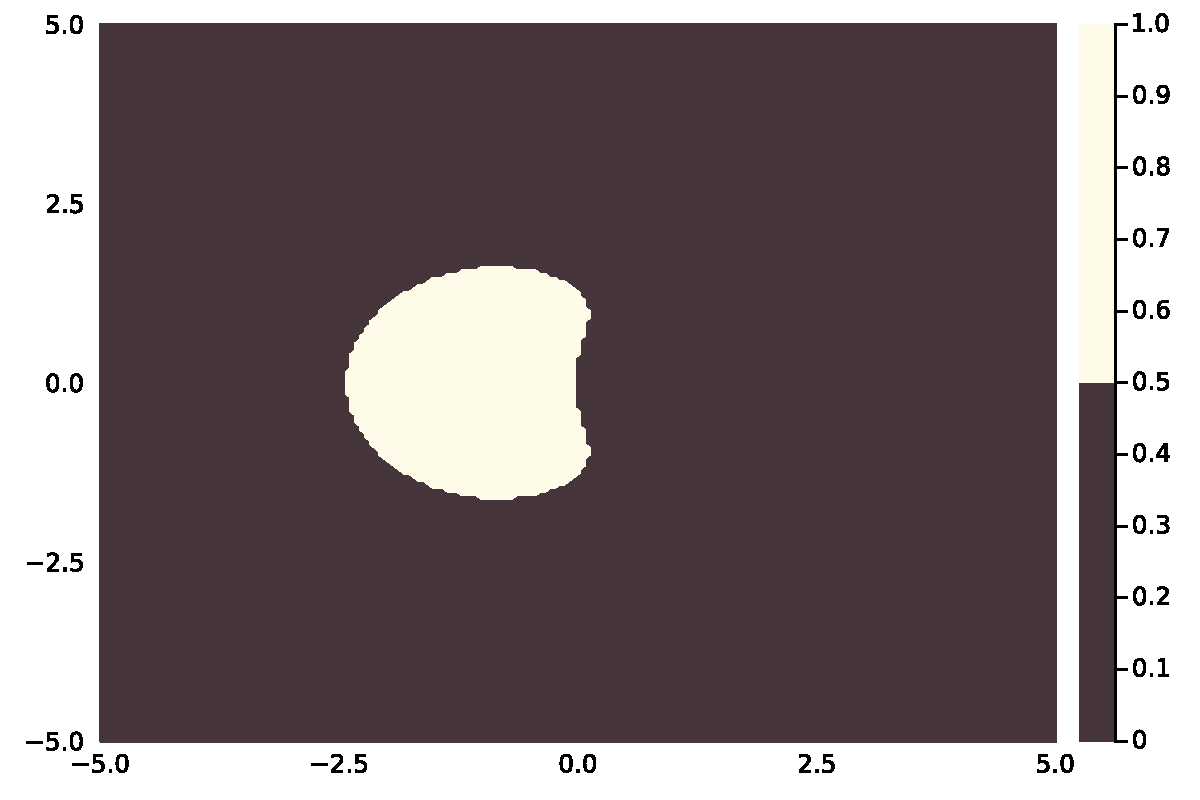
\includegraphics[width=\linewidth]{figures/ass_4_report_2_1.pdf}

\subsection{2-step 4th order LMM}

\begin{lstlisting}
(*@\HLJLcs{{\#}}@*) (*@\HLJLcs{2-step}@*) (*@\HLJLcs{4th}@*) (*@\HLJLcs{order}@*) (*@\HLJLcs{LMM}@*)
(*@\HLJLn{\ensuremath{\alpha}}@*) (*@\HLJLoB{=}@*) (*@\HLJLp{[}@*)(*@\HLJLoB{-}@*)(*@\HLJLnfB{1.0}@*)(*@\HLJLp{,}@*) (*@\HLJLnfB{0.0}@*)(*@\HLJLp{,}@*) (*@\HLJLnfB{1.0}@*)(*@\HLJLp{];}@*) (*@\HLJLn{\ensuremath{\beta}}@*) (*@\HLJLoB{=}@*) (*@\HLJLp{[}@*)(*@\HLJLni{1}@*)(*@\HLJLoB{/}@*)(*@\HLJLni{3}@*)(*@\HLJLp{,}@*) (*@\HLJLni{4}@*)(*@\HLJLoB{/}@*)(*@\HLJLni{3}@*)(*@\HLJLp{,}@*) (*@\HLJLni{1}@*)(*@\HLJLoB{/}@*)(*@\HLJLni{3}@*)(*@\HLJLp{];}@*)
(*@\HLJLn{xs}@*)(*@\HLJLp{,}@*)(*@\HLJLn{Z}@*) (*@\HLJLoB{=}@*) (*@\HLJLnf{RASlmm}@*)(*@\HLJLp{(}@*)(*@\HLJLn{\ensuremath{\alpha}}@*)(*@\HLJLp{,}@*) (*@\HLJLn{\ensuremath{\beta}}@*)(*@\HLJLp{)}@*)

(*@\HLJLnf{contourf}@*)(*@\HLJLp{(}@*)(*@\HLJLn{xs}@*)(*@\HLJLp{,}@*) (*@\HLJLn{xs}@*)(*@\HLJLp{,}@*) (*@\HLJLn{Z}@*)(*@\HLJLp{,}@*) (*@\HLJLn{levels}@*) (*@\HLJLoB{=}@*) (*@\HLJLni{1}@*)(*@\HLJLp{)}@*)
\end{lstlisting}

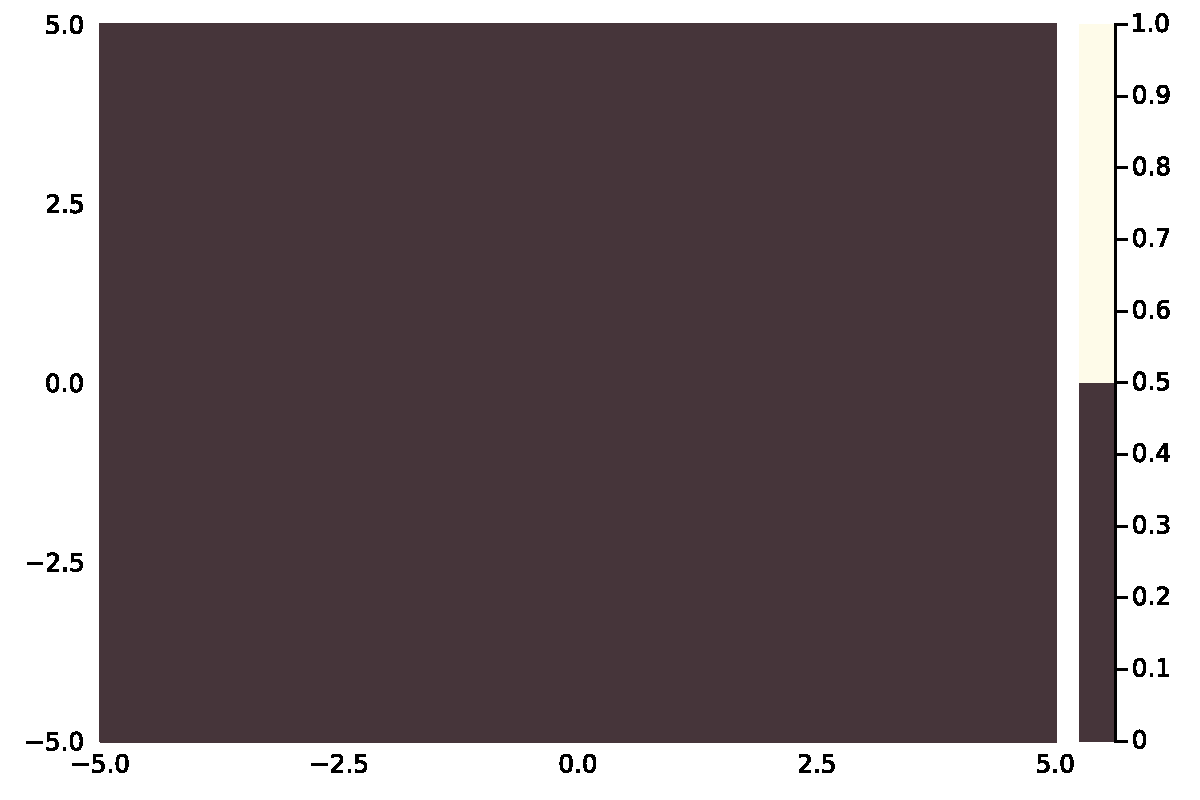
\includegraphics[width=\linewidth]{figures/ass_4_report_3_1.pdf}

\subsection{2-step BDF (BDF2)}

\begin{lstlisting}
(*@\HLJLcs{{\#}}@*) (*@\HLJLcs{2-step}@*) (*@\HLJLcs{BDF}@*) (*@\HLJLcs{(BDF2)}@*)
(*@\HLJLn{\ensuremath{\alpha}}@*) (*@\HLJLoB{=}@*) (*@\HLJLp{[}@*)(*@\HLJLni{1}@*)(*@\HLJLoB{/}@*)(*@\HLJLni{2}@*)(*@\HLJLp{,}@*) (*@\HLJLoB{-}@*)(*@\HLJLnfB{2.0}@*)(*@\HLJLp{,}@*) (*@\HLJLni{3}@*)(*@\HLJLoB{/}@*)(*@\HLJLni{2}@*)(*@\HLJLp{];}@*) (*@\HLJLn{\ensuremath{\beta}}@*) (*@\HLJLoB{=}@*) (*@\HLJLp{[}@*)(*@\HLJLnfB{0.0}@*)(*@\HLJLp{,}@*) (*@\HLJLnfB{0.0}@*)(*@\HLJLp{,}@*) (*@\HLJLnfB{1.0}@*)(*@\HLJLp{];}@*)
(*@\HLJLn{xs}@*)(*@\HLJLp{,}@*)(*@\HLJLn{Z}@*) (*@\HLJLoB{=}@*) (*@\HLJLnf{RASlmm}@*)(*@\HLJLp{(}@*)(*@\HLJLn{\ensuremath{\alpha}}@*)(*@\HLJLp{,}@*) (*@\HLJLn{\ensuremath{\beta}}@*)(*@\HLJLp{)}@*)

(*@\HLJLnf{contourf}@*)(*@\HLJLp{(}@*)(*@\HLJLn{xs}@*)(*@\HLJLp{,}@*) (*@\HLJLn{xs}@*)(*@\HLJLp{,}@*) (*@\HLJLn{Z}@*)(*@\HLJLp{,}@*) (*@\HLJLn{levels}@*) (*@\HLJLoB{=}@*) (*@\HLJLni{1}@*)(*@\HLJLp{)}@*)
\end{lstlisting}

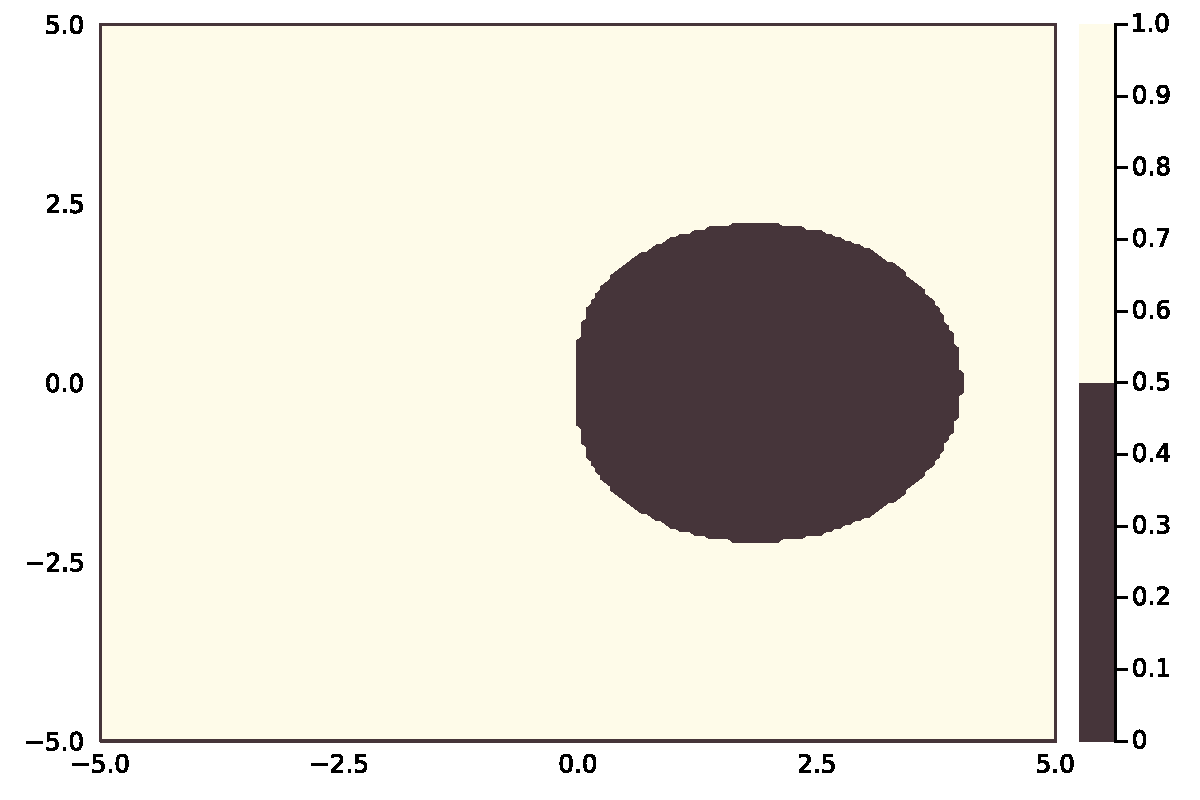
\includegraphics[width=\linewidth]{figures/ass_4_report_4_1.pdf}

\subsection{3-step BDF (BDF3)}

\begin{lstlisting}
(*@\HLJLcs{{\#}}@*) (*@\HLJLcs{3-step}@*) (*@\HLJLcs{BDF}@*) (*@\HLJLcs{(BDF3)}@*)
(*@\HLJLn{\ensuremath{\alpha}}@*) (*@\HLJLoB{=}@*) (*@\HLJLp{[}@*)(*@\HLJLoB{-}@*)(*@\HLJLni{1}@*)(*@\HLJLoB{/}@*)(*@\HLJLni{3}@*)(*@\HLJLp{,}@*) (*@\HLJLni{3}@*)(*@\HLJLoB{/}@*)(*@\HLJLni{2}@*)(*@\HLJLp{,}@*) (*@\HLJLoB{-}@*)(*@\HLJLnfB{3.0}@*)(*@\HLJLp{,}@*) (*@\HLJLni{11}@*)(*@\HLJLoB{/}@*)(*@\HLJLni{6}@*)(*@\HLJLp{];}@*) (*@\HLJLn{\ensuremath{\beta}}@*) (*@\HLJLoB{=}@*) (*@\HLJLp{[}@*)(*@\HLJLnfB{0.0}@*)(*@\HLJLp{,}@*) (*@\HLJLnfB{0.0}@*)(*@\HLJLp{,}@*) (*@\HLJLnfB{0.0}@*)(*@\HLJLp{,}@*) (*@\HLJLnfB{1.0}@*)(*@\HLJLp{];}@*)
(*@\HLJLn{xs}@*)(*@\HLJLp{,}@*)(*@\HLJLn{Z}@*) (*@\HLJLoB{=}@*) (*@\HLJLnf{RASlmm}@*)(*@\HLJLp{(}@*)(*@\HLJLn{\ensuremath{\alpha}}@*)(*@\HLJLp{,}@*) (*@\HLJLn{\ensuremath{\beta}}@*)(*@\HLJLp{)}@*)

(*@\HLJLnf{contourf}@*)(*@\HLJLp{(}@*)(*@\HLJLn{xs}@*)(*@\HLJLp{,}@*) (*@\HLJLn{xs}@*)(*@\HLJLp{,}@*) (*@\HLJLn{Z}@*)(*@\HLJLp{,}@*) (*@\HLJLn{levels}@*) (*@\HLJLoB{=}@*) (*@\HLJLni{1}@*)(*@\HLJLp{)}@*)
\end{lstlisting}

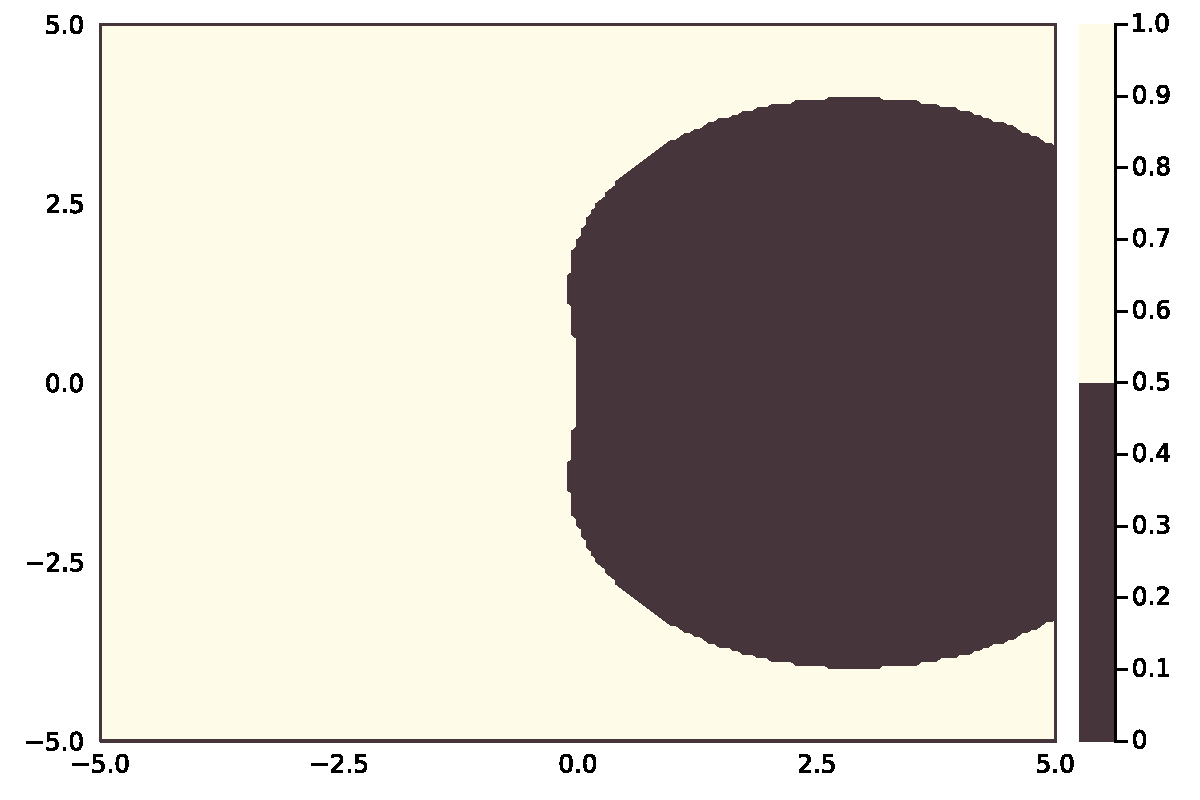
\includegraphics[width=\linewidth]{figures/ass_4_report_5_1.pdf}

\section{Problem 3: Shooting Method}

\begin{lstlisting}
(*@\HLJLcs{{\#}}@*) (*@\HLJLcs{Differential}@*) (*@\HLJLcs{equation}@*)
(*@\HLJLnf{f}@*)(*@\HLJLp{(}@*)(*@\HLJLn{u}@*)(*@\HLJLp{,}@*) (*@\HLJLn{x}@*)(*@\HLJLp{,}@*) (*@\HLJLn{\ensuremath{\mu}}@*)(*@\HLJLp{)}@*) (*@\HLJLoB{=}@*) (*@\HLJLp{[}@*)(*@\HLJLn{u}@*)(*@\HLJLp{[}@*)(*@\HLJLni{2}@*)(*@\HLJLp{];}@*) (*@\HLJLnf{sin}@*)(*@\HLJLp{(}@*)(*@\HLJLn{x}@*)(*@\HLJLp{)}@*) (*@\HLJLoB{+}@*) (*@\HLJLp{(}@*)(*@\HLJLni{1}@*)(*@\HLJLoB{+}@*)(*@\HLJLnfB{0.5}@*)(*@\HLJLoB{*}@*)(*@\HLJLn{u}@*)(*@\HLJLp{[}@*)(*@\HLJLni{2}@*)(*@\HLJLp{]}@*)(*@\HLJLoB{{\textasciicircum}}@*)(*@\HLJLni{2}@*)(*@\HLJLp{)}@*)(*@\HLJLoB{*}@*)(*@\HLJLn{u}@*)(*@\HLJLp{[}@*)(*@\HLJLni{1}@*)(*@\HLJLp{]]}@*)

(*@\HLJLcs{{\#}}@*) (*@\HLJLcs{BVP}@*) (*@\HLJLcs{conditions}@*)
(*@\HLJLn{a}@*) (*@\HLJLoB{=}@*) (*@\HLJLnfB{0.0}@*)(*@\HLJLp{;}@*) (*@\HLJLn{b}@*) (*@\HLJLoB{=}@*) (*@\HLJLnfB{2.0}@*)(*@\HLJLp{;}@*) (*@\HLJLn{\ensuremath{\alpha}}@*) (*@\HLJLoB{=}@*) (*@\HLJLni{1}@*)(*@\HLJLp{;}@*) (*@\HLJLn{\ensuremath{\beta}}@*) (*@\HLJLoB{=}@*) (*@\HLJLnfB{0.5}@*)(*@\HLJLp{;}@*)

(*@\HLJLcs{{\#}}@*) (*@\HLJLcs{Variables}@*)
(*@\HLJLn{h}@*) (*@\HLJLoB{=}@*) (*@\HLJLnfB{0.002}@*)(*@\HLJLp{;}@*) (*@\HLJLn{T}@*) (*@\HLJLoB{=}@*) (*@\HLJLn{b}@*)(*@\HLJLoB{-}@*)(*@\HLJLn{a}@*)(*@\HLJLp{;}@*) (*@\HLJLn{N}@*) (*@\HLJLoB{=}@*) (*@\HLJLnf{Int}@*)(*@\HLJLp{(}@*)(*@\HLJLn{T}@*)(*@\HLJLoB{/}@*)(*@\HLJLn{h}@*)(*@\HLJLp{);}@*)

(*@\HLJLcs{{\#}}@*) (*@\HLJLcs{Find}@*) (*@\HLJLcs{\ensuremath{\nu}}@*) (*@\HLJLcs{for}@*) (*@\HLJLcs{IVP}@*)
(*@\HLJLcs{{\#}}@*) (*@\HLJLcs{\ensuremath{\nu}}@*) (*@\HLJLcs{=}@*) (*@\HLJLcs{(\ensuremath{\beta}}@*) (*@\HLJLcs{-}@*) (*@\HLJLcs{\ensuremath{\alpha})/(b-a)}@*) (*@\HLJLcs{{\#}}@*) (*@\HLJLcs{guess}@*) (*@\HLJLcs{slope}@*) (*@\HLJLcs{avg}@*) (*@\HLJLcs{rate}@*) (*@\HLJLcs{of}@*) (*@\HLJLcs{change}@*) (*@\HLJLcs{over}@*) (*@\HLJLcs{interval}@*)
(*@\HLJLn{\ensuremath{\nu}}@*) (*@\HLJLoB{=}@*) (*@\HLJLoB{-}@*)(*@\HLJLnfB{1.0}@*)

(*@\HLJLk{function}@*) (*@\HLJLnf{G}@*)(*@\HLJLp{(}@*)(*@\HLJLn{\ensuremath{\nu}}@*)(*@\HLJLp{)}@*)
    (*@\HLJLn{u0}@*) (*@\HLJLoB{=}@*) (*@\HLJLp{[}@*)(*@\HLJLn{\ensuremath{\alpha}}@*)(*@\HLJLp{;}@*) (*@\HLJLn{\ensuremath{\nu}}@*)(*@\HLJLp{]}@*)
    (*@\HLJLn{u}@*) (*@\HLJLoB{=}@*) (*@\HLJLnf{rk4}@*)(*@\HLJLp{(}@*)(*@\HLJLn{f}@*)(*@\HLJLp{,}@*) (*@\HLJLn{N}@*)(*@\HLJLp{,}@*) (*@\HLJLn{T}@*)(*@\HLJLp{,}@*) (*@\HLJLn{u0}@*)(*@\HLJLp{)}@*)
    (*@\HLJLk{return}@*) (*@\HLJLn{u}@*)(*@\HLJLp{[}@*)(*@\HLJLni{1}@*)(*@\HLJLp{,}@*)(*@\HLJLk{end}@*)(*@\HLJLp{]}@*) (*@\HLJLoB{-}@*) (*@\HLJLn{\ensuremath{\beta}}@*)
(*@\HLJLk{end}@*)

(*@\HLJLn{\ensuremath{\nu}}@*) (*@\HLJLoB{=}@*) (*@\HLJLnf{Newtons{\_}n}@*)(*@\HLJLp{(}@*)(*@\HLJLn{G}@*)(*@\HLJLp{,}@*) (*@\HLJLn{\ensuremath{\nu}}@*)(*@\HLJLp{,}@*) (*@\HLJLnfB{0.0}@*)(*@\HLJLp{)}@*)
\end{lstlisting}

\begin{lstlisting}
-1.4850899639208666
\end{lstlisting}


\begin{lstlisting}
(*@\HLJLcs{{\#}}@*) (*@\HLJLcs{Solve}@*) (*@\HLJLcs{ode}@*) (*@\HLJLcs{using}@*) (*@\HLJLcs{\ensuremath{\nu}}@*) (*@\HLJLcs{found}@*) (*@\HLJLcs{above}@*)
(*@\HLJLn{u0}@*) (*@\HLJLoB{=}@*) (*@\HLJLp{[}@*)(*@\HLJLn{\ensuremath{\alpha}}@*)(*@\HLJLp{;}@*) (*@\HLJLn{\ensuremath{\nu}}@*)(*@\HLJLp{]}@*)
(*@\HLJLn{u}@*) (*@\HLJLoB{=}@*) (*@\HLJLnf{rk4}@*)(*@\HLJLp{(}@*)(*@\HLJLn{f}@*)(*@\HLJLp{,}@*) (*@\HLJLn{N}@*)(*@\HLJLp{,}@*) (*@\HLJLn{T}@*)(*@\HLJLp{,}@*) (*@\HLJLn{u0}@*)(*@\HLJLp{)}@*)

(*@\HLJLn{t}@*) (*@\HLJLoB{=}@*) (*@\HLJLnf{collect}@*)(*@\HLJLp{(}@*)(*@\HLJLni{0}@*)(*@\HLJLoB{:}@*)(*@\HLJLn{N}@*)(*@\HLJLp{)}@*)(*@\HLJLoB{*}@*)(*@\HLJLn{h}@*)
(*@\HLJLnf{plot}@*)(*@\HLJLp{(}@*)(*@\HLJLn{t}@*)(*@\HLJLp{,}@*) (*@\HLJLn{u}@*)(*@\HLJLp{[}@*)(*@\HLJLni{1}@*)(*@\HLJLp{,}@*)(*@\HLJLoB{:}@*)(*@\HLJLp{])}@*)
\end{lstlisting}

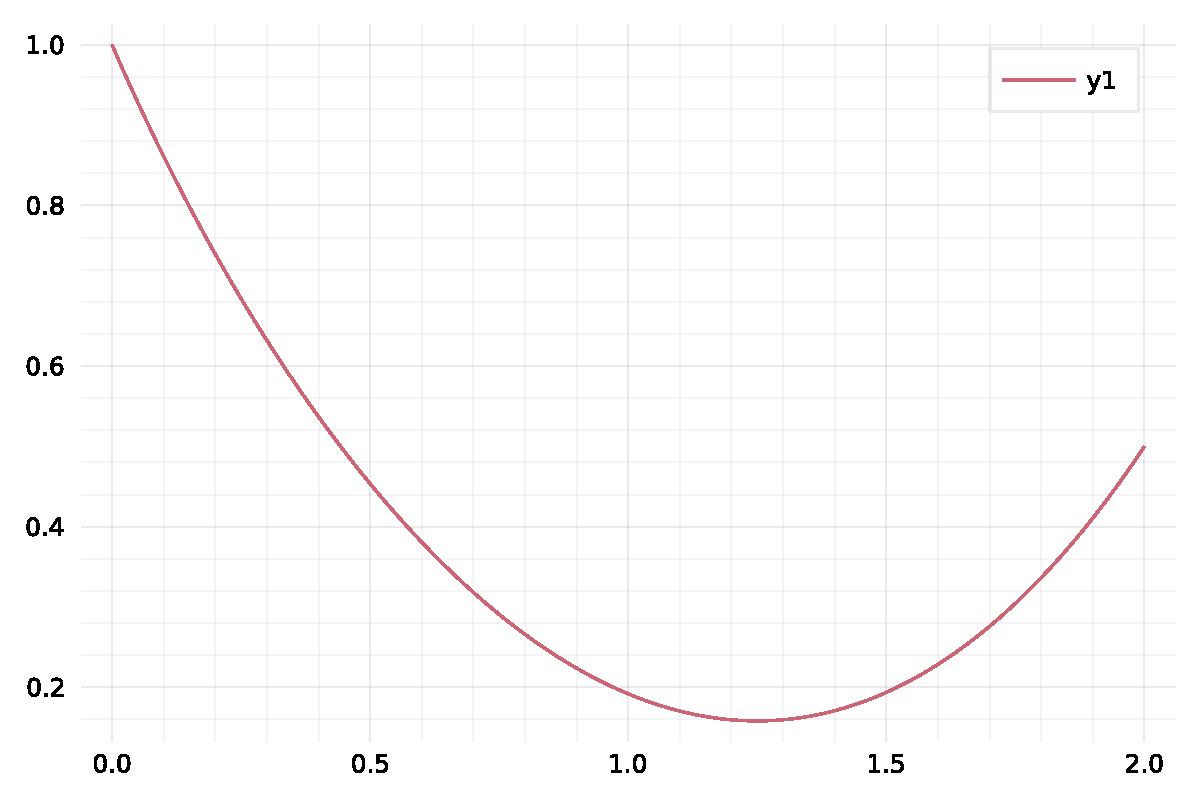
\includegraphics[width=\linewidth]{figures/ass_4_report_7_1.pdf}

\section{Problem 4: FDM}

\begin{lstlisting}
(*@\HLJLn{T}@*) (*@\HLJLoB{=}@*) (*@\HLJLnfB{2.0}@*)(*@\HLJLp{;}@*) (*@\HLJLn{N}@*) (*@\HLJLoB{=}@*) (*@\HLJLni{1000}@*)(*@\HLJLp{;}@*) (*@\HLJLn{h}@*) (*@\HLJLoB{=}@*) (*@\HLJLn{T}@*) (*@\HLJLoB{/}@*) (*@\HLJLn{N}@*)
(*@\HLJLn{x}@*) (*@\HLJLoB{=}@*) (*@\HLJLnf{collect}@*)(*@\HLJLp{(}@*)(*@\HLJLni{0}@*)(*@\HLJLoB{:}@*)(*@\HLJLn{N}@*)(*@\HLJLoB{-}@*)(*@\HLJLni{1}@*)(*@\HLJLp{)}@*)(*@\HLJLoB{*}@*)(*@\HLJLn{h}@*)

(*@\HLJLcs{{\#}}@*) (*@\HLJLcs{Laplacian}@*)
(*@\HLJLn{L}@*) (*@\HLJLoB{=}@*) (*@\HLJLni{1}@*)(*@\HLJLoB{/}@*)(*@\HLJLn{h}@*)(*@\HLJLoB{{\textasciicircum}}@*)(*@\HLJLni{2}@*) (*@\HLJLoB{*}@*) (*@\HLJLnf{spdiagm}@*)(*@\HLJLp{(}@*)(*@\HLJLoB{-}@*)(*@\HLJLni{1}@*)(*@\HLJLoB{=>}@*)(*@\HLJLnf{ones}@*)(*@\HLJLp{(}@*)(*@\HLJLn{N}@*)(*@\HLJLoB{-}@*)(*@\HLJLni{1}@*)(*@\HLJLp{),}@*)(*@\HLJLni{0}@*)(*@\HLJLoB{=>-}@*)(*@\HLJLnfB{2.0}@*)(*@\HLJLoB{*}@*)(*@\HLJLnf{ones}@*)(*@\HLJLp{(}@*)(*@\HLJLn{N}@*)(*@\HLJLp{),}@*)(*@\HLJLni{1}@*)(*@\HLJLoB{=>}@*)(*@\HLJLnf{ones}@*)(*@\HLJLp{(}@*)(*@\HLJLn{N}@*)(*@\HLJLoB{-}@*)(*@\HLJLni{1}@*)(*@\HLJLp{))}@*)

(*@\HLJLcs{{\#}}@*) (*@\HLJLcs{Differential}@*) (*@\HLJLcs{equation}@*)
(*@\HLJLn{\ensuremath{\alpha}}@*) (*@\HLJLoB{=}@*) (*@\HLJLni{1}@*)(*@\HLJLp{;}@*) (*@\HLJLn{\ensuremath{\beta}}@*) (*@\HLJLoB{=}@*) (*@\HLJLni{1}@*)(*@\HLJLp{;}@*)
(*@\HLJLn{g}@*) (*@\HLJLoB{=}@*) (*@\HLJLoB{-}@*)(*@\HLJLni{625}@*)(*@\HLJLoB{*}@*)(*@\HLJLn{x}@*)(*@\HLJLp{;}@*)

(*@\HLJLcs{{\#}}@*) (*@\HLJLcs{Boundary}@*) (*@\HLJLcs{conditions}@*)
(*@\HLJLn{g}@*)(*@\HLJLp{[}@*)(*@\HLJLni{1}@*)(*@\HLJLp{]}@*) (*@\HLJLoB{=}@*) (*@\HLJLn{g}@*)(*@\HLJLp{[}@*)(*@\HLJLni{1}@*)(*@\HLJLp{]}@*) (*@\HLJLoB{-}@*) (*@\HLJLp{(}@*)(*@\HLJLni{1}@*)(*@\HLJLoB{/}@*)(*@\HLJLn{h}@*)(*@\HLJLoB{{\textasciicircum}}@*)(*@\HLJLni{2}@*)(*@\HLJLp{)}@*)(*@\HLJLoB{*}@*)(*@\HLJLn{\ensuremath{\alpha}}@*)
(*@\HLJLn{g}@*)(*@\HLJLp{[}@*)(*@\HLJLn{N}@*)(*@\HLJLp{]}@*) (*@\HLJLoB{=}@*) (*@\HLJLn{g}@*)(*@\HLJLp{[}@*)(*@\HLJLn{N}@*)(*@\HLJLp{]}@*) (*@\HLJLoB{-}@*) (*@\HLJLp{(}@*)(*@\HLJLni{1}@*)(*@\HLJLoB{/}@*)(*@\HLJLn{h}@*)(*@\HLJLoB{{\textasciicircum}}@*)(*@\HLJLni{2}@*)(*@\HLJLp{)}@*)(*@\HLJLoB{*}@*)(*@\HLJLn{\ensuremath{\beta}}@*)

(*@\HLJLn{u}@*) (*@\HLJLoB{=}@*) (*@\HLJLp{(}@*)(*@\HLJLn{L}@*) (*@\HLJLoB{-}@*) (*@\HLJLni{625}@*)(*@\HLJLoB{*}@*)(*@\HLJLn{I}@*)(*@\HLJLp{)}@*)(*@\HLJLoB{{\textbackslash}}@*)(*@\HLJLn{g}@*)

(*@\HLJLnf{u{\_}exact}@*)(*@\HLJLp{(}@*)(*@\HLJLn{x}@*)(*@\HLJLp{)}@*) (*@\HLJLoB{=}@*) (*@\HLJLn{x}@*) (*@\HLJLoB{+}@*) (*@\HLJLp{(}@*)(*@\HLJLni{1}@*)(*@\HLJLoB{+}@*)(*@\HLJLnf{exp}@*)(*@\HLJLp{(}@*)(*@\HLJLoB{-}@*)(*@\HLJLni{50}@*)(*@\HLJLp{))}@*)(*@\HLJLoB{/}@*)(*@\HLJLp{(}@*)(*@\HLJLni{1}@*)(*@\HLJLoB{-}@*)(*@\HLJLnf{exp}@*)(*@\HLJLp{(}@*)(*@\HLJLoB{-}@*)(*@\HLJLni{100}@*)(*@\HLJLp{))}@*)(*@\HLJLoB{*}@*)(*@\HLJLp{(}@*)(*@\HLJLn{exp}@*)(*@\HLJLoB{.}@*)(*@\HLJLp{(}@*)(*@\HLJLoB{-}@*)(*@\HLJLni{25}@*)(*@\HLJLoB{*}@*)(*@\HLJLn{x}@*)(*@\HLJLp{)}@*) (*@\HLJLoB{-}@*) (*@\HLJLn{exp}@*)(*@\HLJLoB{.}@*)(*@\HLJLp{(}@*)(*@\HLJLni{25}@*)(*@\HLJLoB{*}@*)(*@\HLJLp{(}@*)(*@\HLJLn{x}@*)(*@\HLJLoB{.-}@*)(*@\HLJLni{2}@*)(*@\HLJLp{)))}@*)
(*@\HLJLnf{plot}@*)(*@\HLJLp{(}@*)(*@\HLJLn{x}@*)(*@\HLJLp{,}@*) (*@\HLJLn{u}@*)(*@\HLJLp{,}@*) (*@\HLJLn{label}@*)(*@\HLJLoB{=}@*)(*@\HLJLs{"{}FDM"{}}@*)(*@\HLJLp{)}@*)
(*@\HLJLnf{plot!}@*)(*@\HLJLp{(}@*)(*@\HLJLn{x}@*)(*@\HLJLp{,}@*)(*@\HLJLnf{u{\_}exact}@*)(*@\HLJLp{(}@*)(*@\HLJLn{x}@*)(*@\HLJLp{),}@*) (*@\HLJLn{label}@*) (*@\HLJLoB{=}@*)(*@\HLJLs{"{}exact"{}}@*)(*@\HLJLp{)}@*)
\end{lstlisting}

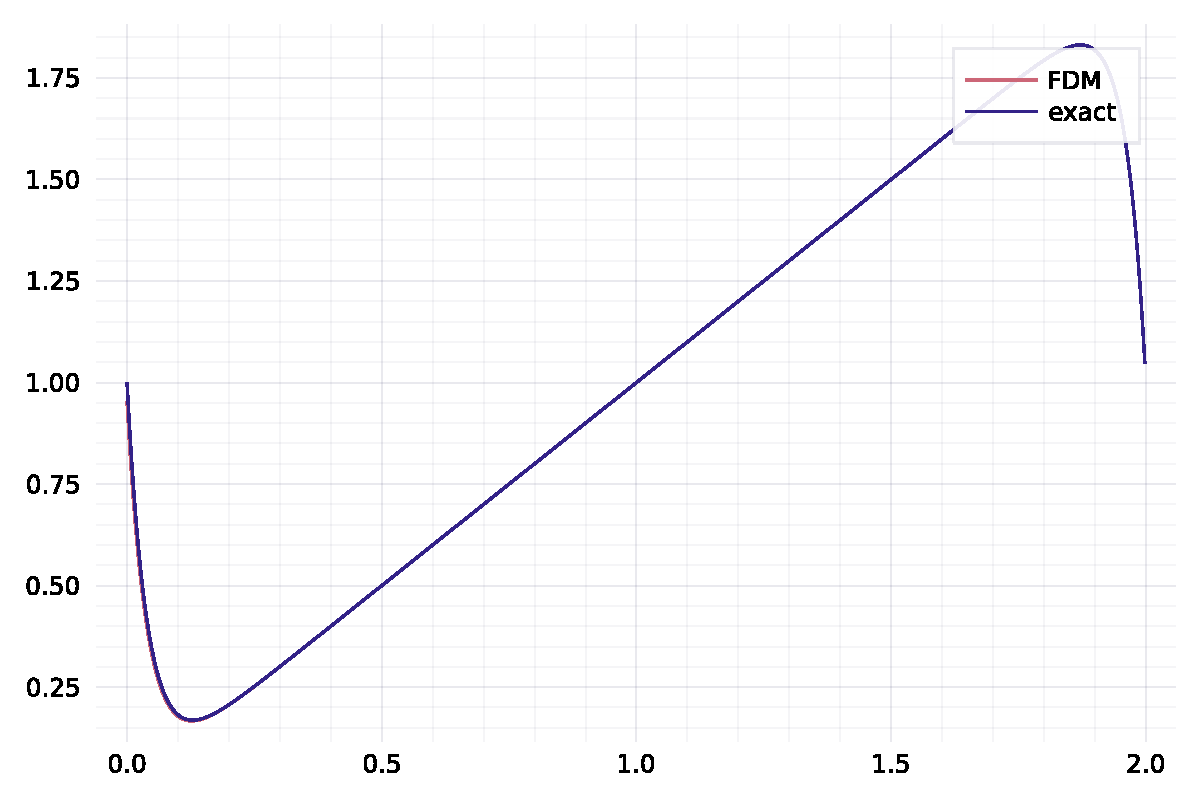
\includegraphics[width=\linewidth]{figures/ass_4_report_8_1.pdf}

\section{Problem 5}

\begin{lstlisting}
(*@\HLJLn{a}@*) (*@\HLJLoB{=}@*) (*@\HLJLnfB{0.0}@*)(*@\HLJLp{;}@*) (*@\HLJLn{b}@*) (*@\HLJLoB{=}@*) (*@\HLJLnfB{2.0}@*)
(*@\HLJLn{T}@*) (*@\HLJLoB{=}@*) (*@\HLJLn{b}@*)(*@\HLJLoB{-}@*)(*@\HLJLn{a}@*)(*@\HLJLp{;}@*) (*@\HLJLn{N}@*) (*@\HLJLoB{=}@*) (*@\HLJLni{1000}@*)(*@\HLJLp{;}@*) 
(*@\HLJLn{h}@*) (*@\HLJLoB{=}@*) (*@\HLJLn{T}@*) (*@\HLJLoB{/}@*) (*@\HLJLp{(}@*)(*@\HLJLn{N}@*)(*@\HLJLoB{-}@*)(*@\HLJLnfB{0.5}@*)(*@\HLJLp{);}@*)
(*@\HLJLn{xs}@*) (*@\HLJLoB{=}@*) (*@\HLJLnf{zeros}@*)(*@\HLJLp{(}@*)(*@\HLJLn{N}@*)(*@\HLJLoB{+}@*)(*@\HLJLni{1}@*)(*@\HLJLp{)}@*)
(*@\HLJLk{for}@*) (*@\HLJLn{i}@*) (*@\HLJLoB{=}@*) (*@\HLJLni{1}@*)(*@\HLJLoB{:}@*)(*@\HLJLn{N}@*)(*@\HLJLoB{+}@*)(*@\HLJLni{1}@*)
    (*@\HLJLn{xs}@*)(*@\HLJLp{[}@*)(*@\HLJLn{i}@*)(*@\HLJLp{]}@*) (*@\HLJLoB{=}@*) (*@\HLJLn{a}@*) (*@\HLJLoB{+}@*) (*@\HLJLp{((}@*)(*@\HLJLn{i}@*)(*@\HLJLoB{-}@*)(*@\HLJLni{1}@*)(*@\HLJLp{)}@*)(*@\HLJLoB{-}@*)(*@\HLJLnfB{0.5}@*)(*@\HLJLp{)}@*)(*@\HLJLoB{*}@*)(*@\HLJLn{h}@*)
(*@\HLJLk{end}@*)

(*@\HLJLcs{{\#}}@*) (*@\HLJLcs{Discretization}@*)
(*@\HLJLn{q}@*) (*@\HLJLoB{=}@*) (*@\HLJLoB{-}@*)(*@\HLJLp{(}@*)(*@\HLJLni{1}@*) (*@\HLJLoB{.+}@*) (*@\HLJLn{exp}@*)(*@\HLJLoB{.}@*)(*@\HLJLp{(}@*)(*@\HLJLoB{-}@*)(*@\HLJLn{sin}@*)(*@\HLJLoB{.}@*)(*@\HLJLp{(}@*)(*@\HLJLn{xs}@*)(*@\HLJLp{)))}@*)
(*@\HLJLn{L}@*) (*@\HLJLoB{=}@*)  (*@\HLJLni{1}@*)(*@\HLJLoB{/}@*)(*@\HLJLn{h}@*)(*@\HLJLoB{{\textasciicircum}}@*)(*@\HLJLni{2}@*) (*@\HLJLoB{*}@*) (*@\HLJLnf{spdiagm}@*)(*@\HLJLp{(}@*)(*@\HLJLoB{-}@*)(*@\HLJLni{1}@*)(*@\HLJLoB{=>}@*)(*@\HLJLnf{ones}@*)(*@\HLJLp{(}@*)(*@\HLJLn{N}@*)(*@\HLJLp{),}@*)(*@\HLJLni{0}@*)(*@\HLJLoB{=>-}@*)(*@\HLJLnfB{2.0}@*)(*@\HLJLoB{*}@*)(*@\HLJLnf{ones}@*)(*@\HLJLp{(}@*)(*@\HLJLn{N}@*)(*@\HLJLoB{+}@*)(*@\HLJLni{1}@*)(*@\HLJLp{),}@*)(*@\HLJLni{1}@*)(*@\HLJLoB{=>}@*)(*@\HLJLnf{ones}@*)(*@\HLJLp{(}@*)(*@\HLJLn{N}@*)(*@\HLJLp{))}@*)
(*@\HLJLn{A}@*) (*@\HLJLoB{=}@*) (*@\HLJLn{L}@*) (*@\HLJLoB{+}@*) (*@\HLJLnf{spdiagm}@*)(*@\HLJLp{(}@*)(*@\HLJLni{0}@*)(*@\HLJLoB{=>}@*)(*@\HLJLn{q}@*)(*@\HLJLp{)}@*)
(*@\HLJLn{A}@*)(*@\HLJLp{[}@*)(*@\HLJLni{1}@*)(*@\HLJLp{,}@*)(*@\HLJLni{1}@*)(*@\HLJLp{]}@*) (*@\HLJLoB{=}@*) (*@\HLJLoB{-}@*)(*@\HLJLni{1}@*)(*@\HLJLoB{/}@*)(*@\HLJLn{h}@*)(*@\HLJLoB{{\textasciicircum}}@*)(*@\HLJLni{2}@*)

(*@\HLJLcs{{\#}}@*) (*@\HLJLcs{Boundary}@*) (*@\HLJLcs{conditions}@*) (*@\HLJLcs{and}@*) (*@\HLJLcs{forcing}@*) (*@\HLJLcs{term}@*) 
(*@\HLJLn{\ensuremath{\alpha}}@*) (*@\HLJLoB{=}@*) (*@\HLJLnfB{2.5}@*)(*@\HLJLp{;}@*) (*@\HLJLn{\ensuremath{\beta}}@*) (*@\HLJLoB{=}@*) (*@\HLJLnfB{0.5}@*)(*@\HLJLp{;}@*)
(*@\HLJLn{g}@*) (*@\HLJLoB{=}@*) (*@\HLJLoB{-}@*)(*@\HLJLni{5}@*) (*@\HLJLoB{.-}@*) (*@\HLJLn{sin}@*)(*@\HLJLoB{.}@*)(*@\HLJLp{(}@*)(*@\HLJLn{xs}@*)(*@\HLJLp{)}@*)(*@\HLJLoB{.{\textasciicircum}}@*)(*@\HLJLni{2}@*)(*@\HLJLp{;}@*)

(*@\HLJLcs{{\#}}@*) (*@\HLJLcs{Incorporate}@*) (*@\HLJLcs{boundary}@*) (*@\HLJLcs{conditions}@*) (*@\HLJLcs{in}@*) (*@\HLJLcs{FDM}@*)
(*@\HLJLn{g}@*)(*@\HLJLp{[}@*)(*@\HLJLni{1}@*)(*@\HLJLp{]}@*) (*@\HLJLoB{=}@*) (*@\HLJLn{g}@*)(*@\HLJLp{[}@*)(*@\HLJLni{1}@*)(*@\HLJLp{]}@*) (*@\HLJLoB{+}@*) (*@\HLJLp{(}@*)(*@\HLJLni{1}@*)(*@\HLJLoB{/}@*)(*@\HLJLn{h}@*)(*@\HLJLp{)}@*)(*@\HLJLoB{*}@*)(*@\HLJLn{\ensuremath{\alpha}}@*)
(*@\HLJLn{g}@*)(*@\HLJLp{[}@*)(*@\HLJLk{end}@*)(*@\HLJLp{]}@*) (*@\HLJLoB{=}@*) (*@\HLJLn{g}@*)(*@\HLJLp{[}@*)(*@\HLJLk{end}@*)(*@\HLJLp{]}@*) (*@\HLJLoB{-}@*) (*@\HLJLp{(}@*)(*@\HLJLni{1}@*)(*@\HLJLoB{/}@*)(*@\HLJLn{h}@*)(*@\HLJLoB{{\textasciicircum}}@*)(*@\HLJLni{2}@*)(*@\HLJLp{)}@*)(*@\HLJLoB{*}@*)(*@\HLJLn{\ensuremath{\beta}}@*)

(*@\HLJLn{u}@*) (*@\HLJLoB{=}@*) (*@\HLJLn{A}@*)(*@\HLJLoB{{\textbackslash}}@*)(*@\HLJLn{g}@*)

(*@\HLJLnf{plot}@*)(*@\HLJLp{(}@*)(*@\HLJLn{xs}@*)(*@\HLJLp{,}@*) (*@\HLJLn{u}@*)(*@\HLJLp{,}@*) (*@\HLJLn{label}@*)(*@\HLJLoB{=}@*)(*@\HLJLs{"{}FDM"{}}@*)(*@\HLJLp{)}@*)

(*@\HLJLcs{{\#}}@*) (*@\HLJLcs{verify}@*) (*@\HLJLcs{solution}@*)
(*@\HLJLnf{f}@*)(*@\HLJLp{(}@*)(*@\HLJLn{u}@*)(*@\HLJLp{,}@*)(*@\HLJLn{x}@*)(*@\HLJLp{,}@*)(*@\HLJLn{\ensuremath{\mu}}@*)(*@\HLJLp{)}@*) (*@\HLJLoB{=}@*) (*@\HLJLp{[}@*)(*@\HLJLn{u}@*)(*@\HLJLp{[}@*)(*@\HLJLni{2}@*)(*@\HLJLp{];}@*) (*@\HLJLoB{-}@*)(*@\HLJLni{5}@*) (*@\HLJLoB{-}@*) (*@\HLJLnf{sin}@*)(*@\HLJLp{(}@*)(*@\HLJLn{x}@*)(*@\HLJLp{)}@*)(*@\HLJLoB{{\textasciicircum}}@*)(*@\HLJLni{2}@*) (*@\HLJLoB{+}@*) (*@\HLJLp{(}@*)(*@\HLJLni{1}@*) (*@\HLJLoB{+}@*) (*@\HLJLnf{exp}@*)(*@\HLJLp{(}@*)(*@\HLJLoB{-}@*)(*@\HLJLnf{sin}@*)(*@\HLJLp{(}@*)(*@\HLJLn{x}@*)(*@\HLJLp{)))}@*)(*@\HLJLoB{*}@*)(*@\HLJLn{u}@*)(*@\HLJLp{[}@*)(*@\HLJLni{1}@*)(*@\HLJLp{]]}@*)
(*@\HLJLn{u0}@*) (*@\HLJLoB{=}@*) (*@\HLJLp{[}@*)(*@\HLJLn{u}@*)(*@\HLJLp{[}@*)(*@\HLJLni{1}@*)(*@\HLJLp{]}@*) (*@\HLJLoB{-}@*) (*@\HLJLn{\ensuremath{\alpha}}@*)(*@\HLJLoB{*}@*)(*@\HLJLn{h}@*)(*@\HLJLoB{/}@*)(*@\HLJLni{2}@*)(*@\HLJLp{;}@*) (*@\HLJLn{\ensuremath{\alpha}}@*)(*@\HLJLp{]}@*)
(*@\HLJLn{u}@*) (*@\HLJLoB{=}@*) (*@\HLJLnf{rk4}@*)(*@\HLJLp{(}@*)(*@\HLJLn{f}@*)(*@\HLJLp{,}@*) (*@\HLJLn{N}@*)(*@\HLJLp{,}@*) (*@\HLJLn{T}@*)(*@\HLJLp{,}@*) (*@\HLJLn{u0}@*)(*@\HLJLp{)}@*)
(*@\HLJLnf{plot!}@*)(*@\HLJLp{(}@*)(*@\HLJLn{xs}@*)(*@\HLJLp{,}@*) (*@\HLJLn{u}@*)(*@\HLJLp{[}@*)(*@\HLJLni{1}@*)(*@\HLJLp{,}@*)(*@\HLJLni{1}@*)(*@\HLJLoB{:}@*)(*@\HLJLn{N}@*)(*@\HLJLoB{+}@*)(*@\HLJLni{1}@*)(*@\HLJLp{],}@*) (*@\HLJLn{label}@*)(*@\HLJLoB{=}@*)(*@\HLJLs{"{}rk4"{}}@*)(*@\HLJLp{)}@*)
\end{lstlisting}

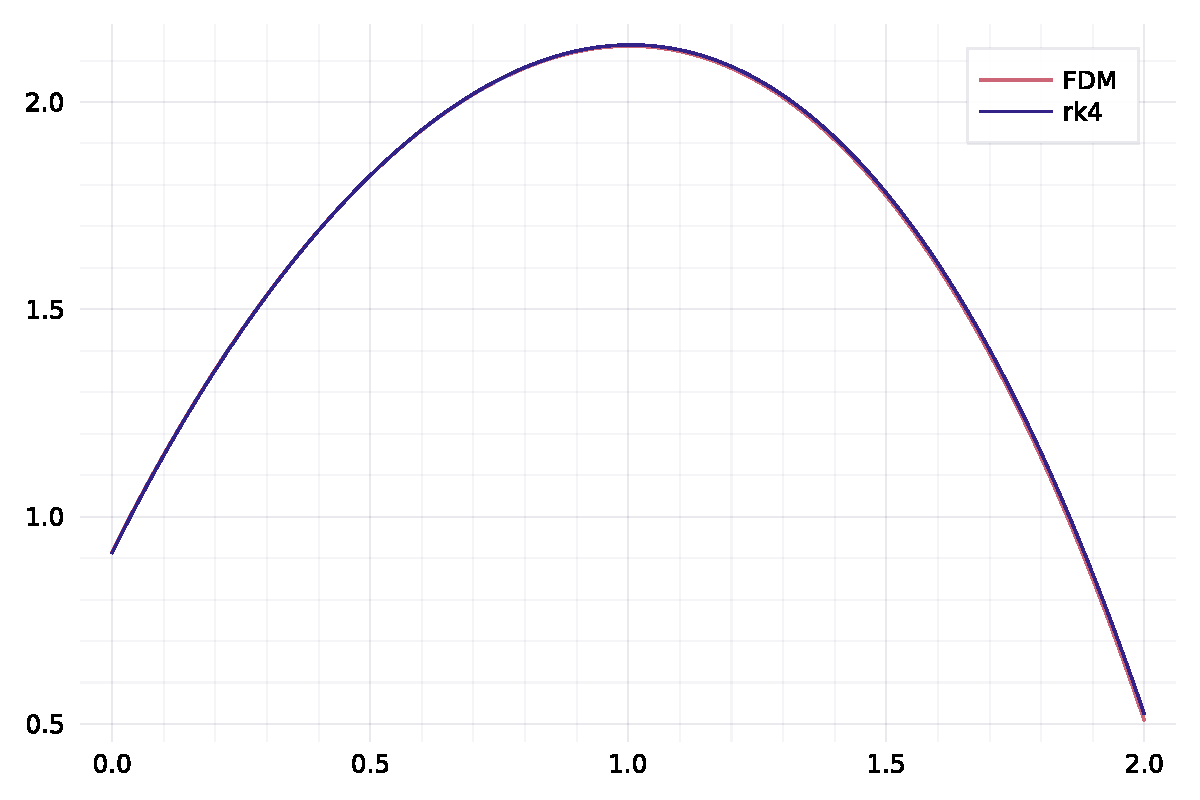
\includegraphics[width=\linewidth]{figures/ass_4_report_9_1.pdf}

\section{Problem 6}

\begin{lstlisting}
(*@\HLJLn{a}@*) (*@\HLJLoB{=}@*) (*@\HLJLnfB{0.0}@*)(*@\HLJLp{;}@*) (*@\HLJLn{b}@*) (*@\HLJLoB{=}@*) (*@\HLJLnfB{2.0}@*)
(*@\HLJLn{T}@*) (*@\HLJLoB{=}@*) (*@\HLJLn{b}@*)(*@\HLJLoB{-}@*)(*@\HLJLn{a}@*)(*@\HLJLp{;}@*) (*@\HLJLn{N}@*) (*@\HLJLoB{=}@*) (*@\HLJLni{1000}@*)(*@\HLJLp{;}@*) (*@\HLJLn{h}@*) (*@\HLJLoB{=}@*) (*@\HLJLn{T}@*) (*@\HLJLoB{/}@*) (*@\HLJLn{N}@*)
(*@\HLJLn{xs}@*) (*@\HLJLoB{=}@*) (*@\HLJLnf{collect}@*)(*@\HLJLp{(}@*)(*@\HLJLni{0}@*)(*@\HLJLoB{:}@*)(*@\HLJLn{N}@*)(*@\HLJLoB{-}@*)(*@\HLJLni{1}@*)(*@\HLJLp{)}@*)(*@\HLJLoB{*}@*)(*@\HLJLn{h}@*)

(*@\HLJLcs{{\#}}@*) (*@\HLJLcs{Discretization}@*)
(*@\HLJLn{q}@*) (*@\HLJLoB{=}@*) (*@\HLJLoB{-}@*)(*@\HLJLp{(}@*)(*@\HLJLni{1}@*) (*@\HLJLoB{.+}@*) (*@\HLJLn{exp}@*)(*@\HLJLoB{.}@*)(*@\HLJLp{(}@*)(*@\HLJLoB{-}@*)(*@\HLJLn{sin}@*)(*@\HLJLoB{.}@*)(*@\HLJLp{(}@*)(*@\HLJLn{xs}@*)(*@\HLJLp{)))}@*)
(*@\HLJLcs{{\#}}@*) (*@\HLJLcs{L}@*) (*@\HLJLcs{=}@*)  (*@\HLJLcs{1/h{\textasciicircum}2}@*) (*@\HLJLcs{*}@*) (*@\HLJLcs{spdiagm(-1=>ones(N),0=>-2.0*ones(N+1),1=>ones(N))}@*)
(*@\HLJLn{L}@*) (*@\HLJLoB{=}@*)  (*@\HLJLni{1}@*)(*@\HLJLoB{/}@*)(*@\HLJLn{h}@*)(*@\HLJLoB{{\textasciicircum}}@*)(*@\HLJLni{2}@*) (*@\HLJLoB{*}@*) (*@\HLJLnf{spdiagm}@*)(*@\HLJLp{(}@*)(*@\HLJLoB{-}@*)(*@\HLJLni{1}@*)(*@\HLJLoB{=>}@*)(*@\HLJLnf{ones}@*)(*@\HLJLp{(}@*)(*@\HLJLn{N}@*)(*@\HLJLoB{-}@*)(*@\HLJLni{1}@*)(*@\HLJLp{),}@*)(*@\HLJLni{0}@*)(*@\HLJLoB{=>-}@*)(*@\HLJLnfB{2.0}@*)(*@\HLJLoB{*}@*)(*@\HLJLnf{ones}@*)(*@\HLJLp{(}@*)(*@\HLJLn{N}@*)(*@\HLJLp{),}@*)(*@\HLJLni{1}@*)(*@\HLJLoB{=>}@*)(*@\HLJLnf{ones}@*)(*@\HLJLp{(}@*)(*@\HLJLn{N}@*)(*@\HLJLoB{-}@*)(*@\HLJLni{1}@*)(*@\HLJLp{))}@*)
(*@\HLJLn{A}@*) (*@\HLJLoB{=}@*) (*@\HLJLn{L}@*) (*@\HLJLoB{+}@*) (*@\HLJLnf{spdiagm}@*)(*@\HLJLp{(}@*)(*@\HLJLni{0}@*)(*@\HLJLoB{=>}@*)(*@\HLJLn{q}@*)(*@\HLJLp{)}@*)

(*@\HLJLcs{{\#}}@*) (*@\HLJLcs{Boundary}@*) (*@\HLJLcs{conditions}@*) (*@\HLJLcs{and}@*) (*@\HLJLcs{forcing}@*) (*@\HLJLcs{term}@*) 
(*@\HLJLn{\ensuremath{\alpha}}@*) (*@\HLJLoB{=}@*) (*@\HLJLnfB{2.5}@*)(*@\HLJLp{;}@*) (*@\HLJLn{\ensuremath{\beta}}@*) (*@\HLJLoB{=}@*) (*@\HLJLnfB{0.5}@*)(*@\HLJLp{;}@*)
(*@\HLJLn{g}@*) (*@\HLJLoB{=}@*) (*@\HLJLoB{-}@*)(*@\HLJLni{5}@*) (*@\HLJLoB{.-}@*) (*@\HLJLn{sin}@*)(*@\HLJLoB{.}@*)(*@\HLJLp{(}@*)(*@\HLJLn{xs}@*)(*@\HLJLp{)}@*)(*@\HLJLoB{.{\textasciicircum}}@*)(*@\HLJLni{2}@*)(*@\HLJLp{;}@*)
(*@\HLJLn{A}@*)(*@\HLJLp{[}@*)(*@\HLJLni{1}@*)(*@\HLJLp{,}@*)(*@\HLJLni{1}@*)(*@\HLJLp{]}@*) (*@\HLJLoB{+=}@*) (*@\HLJLp{(}@*)(*@\HLJLni{1}@*)(*@\HLJLoB{/}@*)(*@\HLJLn{h}@*)(*@\HLJLoB{{\textasciicircum}}@*)(*@\HLJLni{2}@*)(*@\HLJLp{)}@*)(*@\HLJLoB{*}@*)(*@\HLJLp{(}@*)(*@\HLJLni{2}@*)(*@\HLJLoB{-}@*)(*@\HLJLn{h}@*)(*@\HLJLp{)}@*)(*@\HLJLoB{/}@*)(*@\HLJLp{(}@*)(*@\HLJLni{2}@*)(*@\HLJLoB{+}@*)(*@\HLJLn{h}@*)(*@\HLJLp{)}@*)

(*@\HLJLcs{{\#}}@*) (*@\HLJLcs{Incorporate}@*) (*@\HLJLcs{boundary}@*) (*@\HLJLcs{conditions}@*) (*@\HLJLcs{in}@*) (*@\HLJLcs{FDM}@*)
(*@\HLJLn{g}@*)(*@\HLJLp{[}@*)(*@\HLJLni{1}@*)(*@\HLJLp{]}@*) (*@\HLJLoB{=}@*) (*@\HLJLn{g}@*)(*@\HLJLp{[}@*)(*@\HLJLni{1}@*)(*@\HLJLp{]}@*) (*@\HLJLoB{-}@*) (*@\HLJLp{(}@*)(*@\HLJLni{1}@*)(*@\HLJLoB{/}@*)(*@\HLJLn{h}@*)(*@\HLJLoB{{\textasciicircum}}@*)(*@\HLJLni{2}@*)(*@\HLJLp{)}@*)(*@\HLJLoB{*}@*)(*@\HLJLni{2}@*)(*@\HLJLoB{*}@*)(*@\HLJLn{\ensuremath{\alpha}}@*)(*@\HLJLoB{*}@*)(*@\HLJLn{h}@*)(*@\HLJLoB{/}@*)(*@\HLJLp{(}@*)(*@\HLJLni{2}@*)(*@\HLJLoB{+}@*)(*@\HLJLn{h}@*)(*@\HLJLp{)}@*)
(*@\HLJLn{g}@*)(*@\HLJLp{[}@*)(*@\HLJLk{end}@*)(*@\HLJLp{]}@*) (*@\HLJLoB{=}@*) (*@\HLJLn{g}@*)(*@\HLJLp{[}@*)(*@\HLJLk{end}@*)(*@\HLJLp{]}@*) (*@\HLJLoB{-}@*) (*@\HLJLp{(}@*)(*@\HLJLni{1}@*)(*@\HLJLoB{/}@*)(*@\HLJLn{h}@*)(*@\HLJLoB{{\textasciicircum}}@*)(*@\HLJLni{2}@*)(*@\HLJLp{)}@*)(*@\HLJLoB{*}@*)(*@\HLJLn{\ensuremath{\beta}}@*)

(*@\HLJLcs{{\#}}@*) (*@\HLJLcs{Solve}@*) (*@\HLJLcs{system}@*)
(*@\HLJLn{u}@*) (*@\HLJLoB{=}@*) (*@\HLJLn{A}@*)(*@\HLJLoB{{\textbackslash}}@*)(*@\HLJLn{g}@*)
(*@\HLJLnf{plot}@*)(*@\HLJLp{(}@*)(*@\HLJLn{xs}@*)(*@\HLJLp{,}@*) (*@\HLJLn{u}@*)(*@\HLJLp{,}@*) (*@\HLJLn{label}@*)(*@\HLJLoB{=}@*)(*@\HLJLs{"{}FDM"{}}@*)(*@\HLJLp{)}@*)

(*@\HLJLcs{{\#}}@*) (*@\HLJLcs{verify}@*) (*@\HLJLcs{solution}@*)
(*@\HLJLnf{f}@*)(*@\HLJLp{(}@*)(*@\HLJLn{u}@*)(*@\HLJLp{,}@*)(*@\HLJLn{x}@*)(*@\HLJLp{,}@*)(*@\HLJLn{\ensuremath{\mu}}@*)(*@\HLJLp{)}@*) (*@\HLJLoB{=}@*) (*@\HLJLp{[}@*)(*@\HLJLn{u}@*)(*@\HLJLp{[}@*)(*@\HLJLni{2}@*)(*@\HLJLp{];}@*) (*@\HLJLoB{-}@*)(*@\HLJLni{5}@*) (*@\HLJLoB{-}@*) (*@\HLJLnf{sin}@*)(*@\HLJLp{(}@*)(*@\HLJLn{x}@*)(*@\HLJLp{)}@*)(*@\HLJLoB{{\textasciicircum}}@*)(*@\HLJLni{2}@*) (*@\HLJLoB{+}@*) (*@\HLJLp{(}@*)(*@\HLJLni{1}@*) (*@\HLJLoB{+}@*) (*@\HLJLnf{exp}@*)(*@\HLJLp{(}@*)(*@\HLJLoB{-}@*)(*@\HLJLnf{sin}@*)(*@\HLJLp{(}@*)(*@\HLJLn{x}@*)(*@\HLJLp{)))}@*)(*@\HLJLoB{*}@*)(*@\HLJLn{u}@*)(*@\HLJLp{[}@*)(*@\HLJLni{1}@*)(*@\HLJLp{]]}@*)
(*@\HLJLn{u0}@*) (*@\HLJLoB{=}@*) (*@\HLJLp{[(}@*)(*@\HLJLni{2}@*)(*@\HLJLoB{*}@*)(*@\HLJLn{\ensuremath{\alpha}}@*)(*@\HLJLoB{*}@*)(*@\HLJLn{h}@*) (*@\HLJLoB{+}@*) (*@\HLJLp{(}@*)(*@\HLJLni{2}@*)(*@\HLJLoB{-}@*)(*@\HLJLn{h}@*)(*@\HLJLp{)}@*)(*@\HLJLoB{*}@*)(*@\HLJLn{u}@*)(*@\HLJLp{[}@*)(*@\HLJLni{1}@*)(*@\HLJLp{])}@*)(*@\HLJLoB{/}@*)(*@\HLJLp{(}@*)(*@\HLJLni{2}@*)(*@\HLJLoB{+}@*)(*@\HLJLn{h}@*)(*@\HLJLp{);}@*) (*@\HLJLni{2}@*)(*@\HLJLoB{*}@*)(*@\HLJLp{(}@*)(*@\HLJLn{u}@*)(*@\HLJLp{[}@*)(*@\HLJLni{1}@*)(*@\HLJLp{]}@*) (*@\HLJLoB{-}@*) (*@\HLJLn{\ensuremath{\alpha}}@*)(*@\HLJLp{)}@*)(*@\HLJLoB{/}@*)(*@\HLJLp{(}@*)(*@\HLJLni{2}@*)(*@\HLJLoB{+}@*)(*@\HLJLn{h}@*)(*@\HLJLp{)]}@*)
(*@\HLJLn{u}@*) (*@\HLJLoB{=}@*) (*@\HLJLnf{rk4}@*)(*@\HLJLp{(}@*)(*@\HLJLn{f}@*)(*@\HLJLp{,}@*) (*@\HLJLn{N}@*)(*@\HLJLp{,}@*) (*@\HLJLn{T}@*)(*@\HLJLp{,}@*) (*@\HLJLn{u0}@*)(*@\HLJLp{)}@*)
(*@\HLJLnf{plot!}@*)(*@\HLJLp{(}@*)(*@\HLJLn{xs}@*)(*@\HLJLp{[}@*)(*@\HLJLni{1}@*)(*@\HLJLoB{:}@*)(*@\HLJLn{N}@*)(*@\HLJLp{],}@*) (*@\HLJLn{u}@*)(*@\HLJLp{[}@*)(*@\HLJLni{1}@*)(*@\HLJLp{,}@*)(*@\HLJLni{1}@*)(*@\HLJLoB{:}@*)(*@\HLJLn{N}@*)(*@\HLJLp{],}@*) (*@\HLJLn{label}@*)(*@\HLJLoB{=}@*)(*@\HLJLs{"{}rk4"{}}@*)(*@\HLJLp{)}@*)
\end{lstlisting}

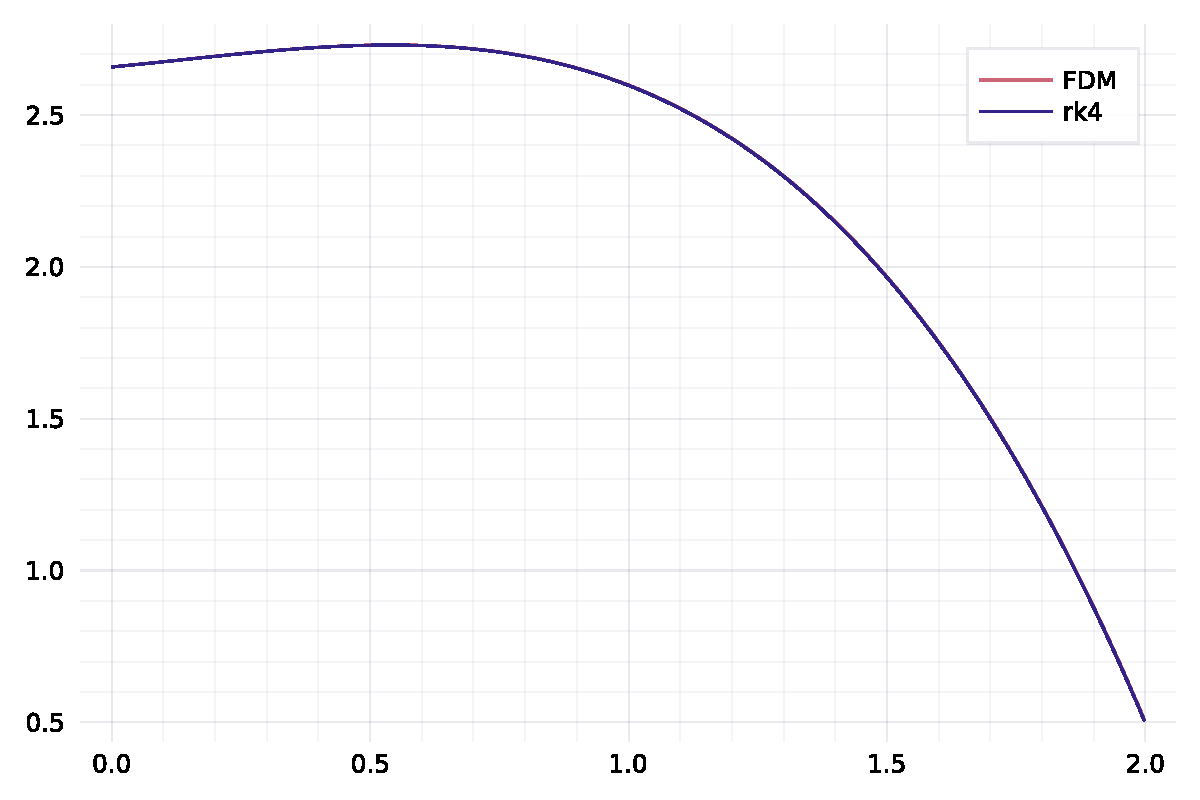
\includegraphics[width=\linewidth]{figures/ass_4_report_10_1.pdf}


\end{document}
